% Data augmentation
%   Image rotation, zoom, shifting, mirroring
%   Possible layer to convert to greyscale to reduce number of params to train
%   Could actually be own section as shared between both models?

% Model walkthrough
%   Final model shape (layer count, params) 
% Total params: 1,045,058
% Trainable params: 1,044,162
% Non-trainable params: 896

%   Hyper-params (and potentially tuning?)
%   approaches to reduce over-fitting (drop-out, regularisation (still need to add))
%   approaches to reduce vanishing gradients (additive layers)
%   approaches to vanishing weights (leaky-relu and normalisation)
%   Distinct CNN layers (for feature extraction) and FCN layers (for classification)
%   probs not image of graph (as massive), but can add to appendix


% Training and learning
%   Time to train, params, layers, etc
%   Learning curves

% Link to colab notebook

\section{Our Model}


\subsection{Architecture}
Our model architecture is shown in Fig \ref{fig:ModelAGraph}. It consists of a shared trunk with two convolutional 
layers with 64 3x3 kernels and relu activation followed by a 2x2 maxpooling layer and a batchnorm layer. It then 
has a convolutional layer with 128 3x3 kernels followed by a 2x2 maxpooling layer. The output of this trunk is 
sent to different branches for age and gender prediction. The age and gender branches have the same architecture
except for the number of filters in their final convodlutional layers. Each branch has two 
convolutional-maxpooling-batchnorm blocks, the first with 64 3x3 convolutional filters and the second with 
128 2x2 filters. They are then followed by another convolutional layer of 64 2x2 filters for gender and 128 2x2 
filters for age. The output of this convolutional layer is then falttened and fed into a 3 layer dense MLP. The first
layer has 128 node, the second 16 and the final layer is a single node for the output. The first and second layers 
use relu activation and the final layer uses no activation for age prediction and a sigmoid activation for gender 
prediction.

\begin{figure}
    \centering
    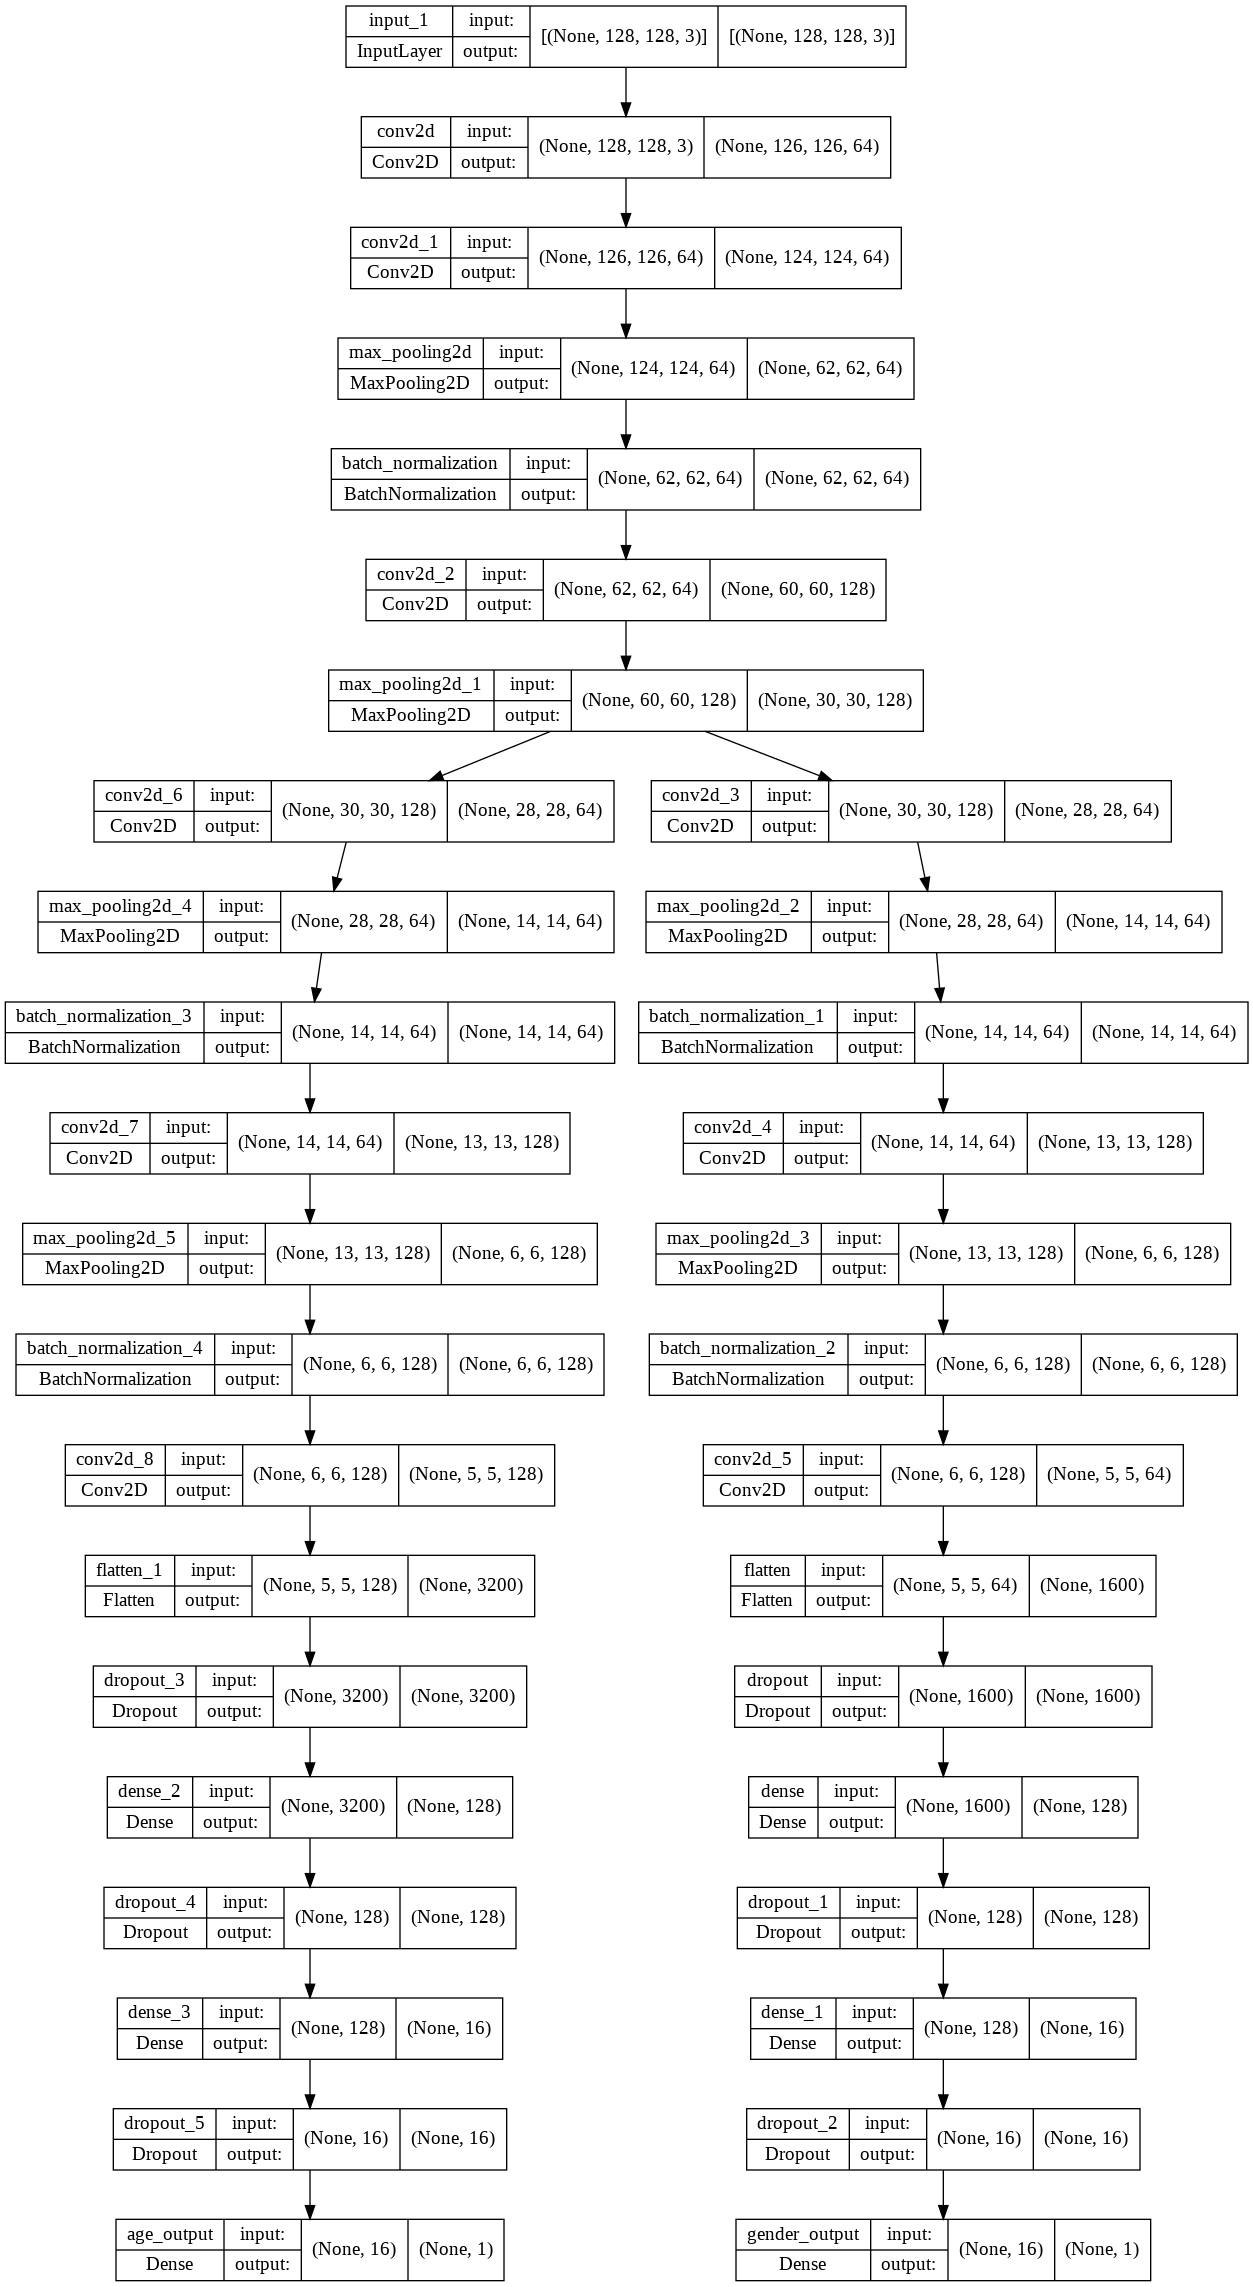
\includegraphics[width=0.7\textwidth]{ModelA_Graph.png}
    \caption{\label{fig:ModelAGraph} The architecture for our model.}
\end{figure}

This architecture was chosen because the first layers of a CNN usually extract generic low-level features which are 
common to many images. Therefore using a shared trunk allows the network to use fewer parameters and helps reduce 
overffitting. The branches then allow the model to further extract higher level features specific to age or gender 
prediction. The batchnorm layers help to reduce overfitting. The dense layers also employ dropout and L2 regularisation
to reduce overffitting. The dropout rate, regulartisation factor and the size of the final convolutional layer in 
the branches were chosen using hyperparameter tuning with keras.tuner.

\subsection{Training}
The model is trained to minimize a weighted average of losses from each branch. The loss for the gender prediction
output is binary cross entropy because it is a binary classification problem and the loss for the age prediction 
is mean squared error because it is a regression problem. Mean squared error was chosen over mean absolute error 
in order to punish large errors more. than small ones. The average loss is weighted 1:50 towards gender prediction
because the average gender losses seen during training were approximately 50 times smaller than the age losses. This 
weighitng was chosen so the model attempts to balance its training objectives without over-prioritising either age or 
gender. The model uses the Adam optimizer with a exponentially decaying learning rate. 

The model is trained for 50 epochs but saves the weights from the epoch with the lowest validation loss. This is 
effectively using early stopping as a means to avoid overfitting.

\subsection{Data}
The model is trained on data from the training data provided. The training data is fed into the model using keras 
data generators. These generators split the data into a training and validation set using a validation split of 0.2. 
Data augmentation is performed to effectively increase the size of the dataset and prevent overfitting. The augmentations
used are rotaion, zoom, and horizontal flipping. The augmentations were performed on both training and validation data.

\subsection{Performance}
The trace of the final training epoch is below.

\begin{verbatim}
    Epoch 50/50
125/125 [==============================] 
- 41s 325ms/step 
- loss: 82.5588 
- age_output_loss: 55.1034 
- gender_output_loss: 0.1627 
- age_output_mean_absolute_error: 5.5780 
- gender_output_binary_accuracy: 0.9330 
- val_loss: 131.3783 
- val_age_output_loss: 90.0434 
- val_gender_output_loss: 0.3111 
- val_age_output_mean_absolute_error: 6.8350 
- val_gender_output_binary_accuracy: 0.8821
\end{verbatim}

Fig \ref{fig:ModelAPerformanceAge} and \ref{fig:ModelAPerformanceGender}
show the training graphs. Our model shows good performance on both age and gender prediction. It achieves an accuracy
of 93\% for gender prediction and a mean absolute error of 5.6 for age prediction on the training data. 
However it can be seen that the model overfits slightly and achieves slightly lower performance on the validation
data, with an accuracy or 88\% for gender prediction and mean absolute error of 6.8 for age prediction. The gender 
branch can be seen to overfit to a greater extent than the age branch.

\begin{figure}
    \centering
    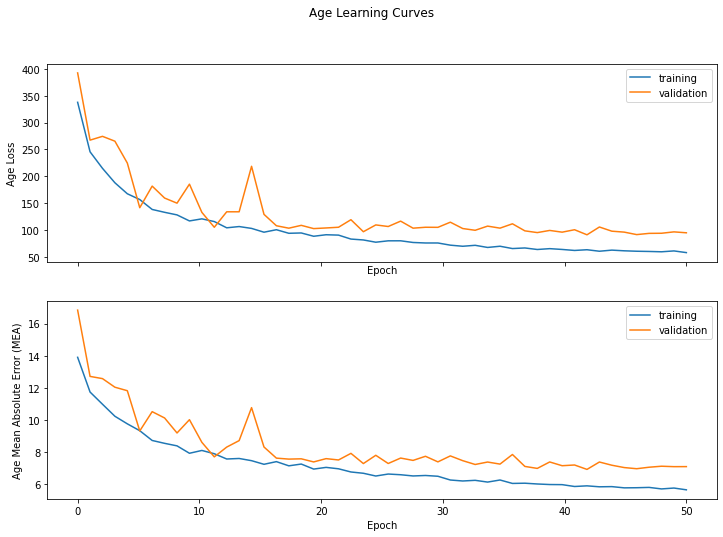
\includegraphics[width=0.7\textwidth]{ModelA_AgeLearning_TunedHyperParams.png}
    \caption{\label{fig:ModelAPerformanceAge} The performance on age prediction for our model.}
\end{figure}


\begin{figure}
    \centering
    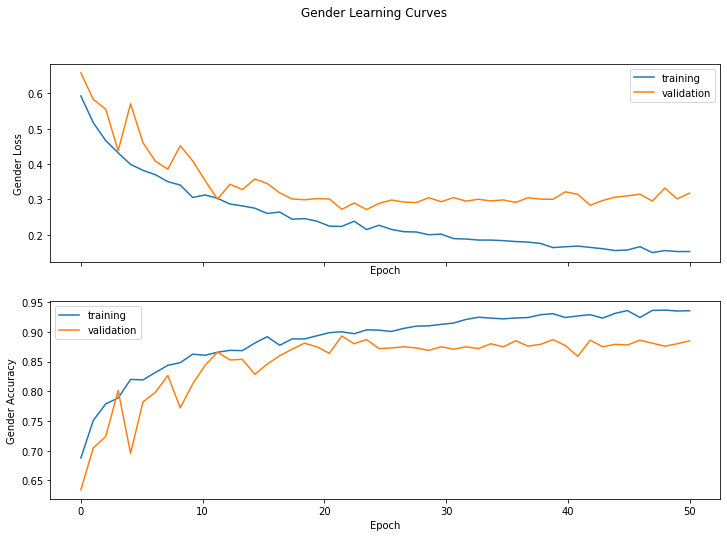
\includegraphics[width=0.7\textwidth]{ModelA_GenderLearning_TunedHyperParams.png}
    \caption{\label{fig:ModelAPerformanceGender} The performance on gender prediction for our model.}
\end{figure}

